\chapter{Current progress}

\label{ch:progress}

\section{\NP{} as puzzles, or one-move games}

Recall that \NP{} is the class of problems solvable by guess-and-check, with a
\emph{check} problem in \P{} (\cref{def:np}):
\[
  \NP = \SetBuilder{L}{
    ∃\underbrace{\mathstrut L'∈\P}_{\mathclap{\text{the ``check'' problem}}} \;
    ∀x \quad
    x∈L ⟺ \underbrace{∃g \; (x, g) ∈ L'}_{\mathclap{\text{guess-and-check}}}
  }.
\]
(In the above, it is \emph{implicitly} required that \(\Abs g\) be
polynomially-bounded with respect to \(\Abs x\), but we have omitted it in
notation for readability.)

Another famous example of a problem in \NP{} is Sudoku, framed as the following
decision problem:
\begin{definition}[\Problem{sudoku}]%
  We are given a square grid with dimensions \(n^2\times n^2\), some of whose
  cells are filled in with numbers in \(\{1,\dotsc,n^2\}\).  Call this grid the
  Sudoku \emph{board}.  The board is evenly partitioned into \(n\) chunks along
  each axis, resulting in \(n^2\) \emph{blocks} each with dimensions \(n\times
  n\).

  Does there exist a way to fill in the rest of the cells so that each row,
  column, and block on the filled-in board contains each number in
  \(\{1,\dotsc,n^2\}\) exactly once?
\end{definition}

\begin{center}
  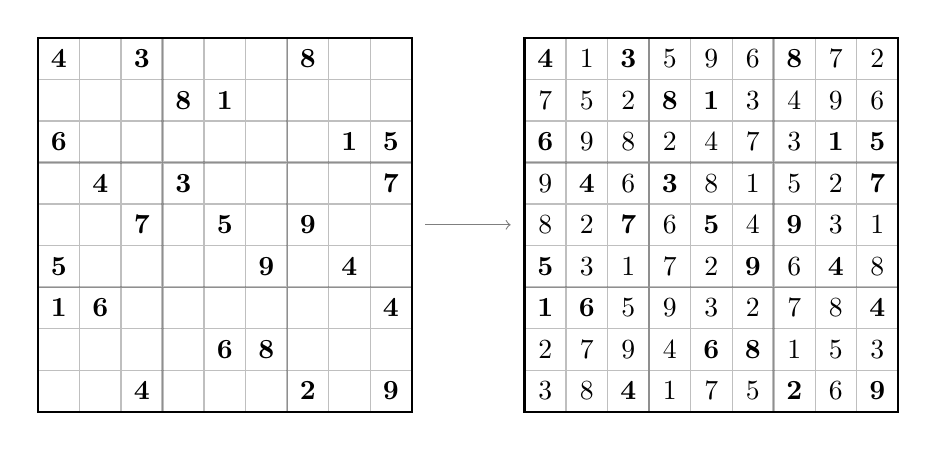
\begin{tikzpicture}[x=3em/2, y=3em/2]
    \tikzset{
      sudoku/.pic={
        \draw[thick] (0,0) rectangle (9,-9);
        \draw[thick, opacity=1/4]
        foreach \i in {3,6} { (0,-\i) -- +(9,0) (\i,0) -- +(0,-9) };
        \draw[opacity=1/4]
        foreach \i in {1,...,8} { (0,-\i) -- +(9,0) (\i,0) -- +(0,-9) };

        \path
        foreach \i in {0,...,8} { foreach \j in {0,...,8} {
            (\j+1/2,-\i-1/2) coordinate(#1-\i-\j)
        } }
        foreach \i/\j/\val in {
          0/0/4,0/2/3,0/6/8,
          1/3/8,1/4/1,
          2/0/6,2/7/1,2/8/5,
          3/1/4,3/3/3,3/8/7,
          4/2/7,4/4/5,4/6/9,
          5/0/5,5/5/9,5/7/4,
          6/0/1,6/1/6,6/8/4,
          7/4/6,7/5/8,
          8/2/4,8/6/2,8/8/9
        } { (#1-\i-\j) node{\(\mathbf\val\)} }
        foreach \i/\j/\name in {4.5/0/w,4.5/9/e} {
          (\j,-\i) coordinate(#1-\name)
        };
      },
    }


    \matrix[column sep=4em]{
      \pic{sudoku=a}; & \pic{sudoku=b}; \\
    };
    \draw[opacity=1/2, arrows={_[sep=1em/2]-To[sep=1em/2]}] (a-e) -- (b-w);

    \path
    foreach \i/\j/\val in {
      0/1/1,0/3/5,0/4/9,0/5/6,0/7/7,0/8/2,
      1/0/7,1/1/5,1/2/2,1/5/3,1/6/4,1/7/9,1/8/6,
      2/1/9,2/2/8,2/3/2,2/4/4,2/5/7,2/6/3,
      3/0/9,3/2/6,3/4/8,3/5/1,3/6/5,3/7/2,
      4/0/8,4/1/2,4/3/6,4/5/4,4/7/3,4/8/1,
      5/1/3,5/2/1,5/3/7,5/4/2,5/6/6,5/8/8,
      6/2/5,6/3/9,6/4/3,6/5/2,6/6/7,6/7/8,
      7/0/2,7/1/7,7/2/9,7/3/4,7/6/1,7/7/5,7/8/3,
      8/0/3,8/1/8,8/3/1,8/4/7,8/5/5,8/7/6
    } { (b-\i-\j) node{\(\val\)} };
  \end{tikzpicture}
\end{center}

For this problem, a ``guess'' \(g\) consists of a list of numbers in
\(\{1,\dotsc,n^2\}\) specifying the values with which to fill in the empty
cells in the given grid.  Then, the ``check'' problem \(L'\) is stated as
follows:
\begin{nested}
  Given a fully-filled-in Sudoku board, does each row, column, and block on the
  grid contain each of \(\{1,\dotsc,n^2\}\) exactly once?
\end{nested}

Sudoku, being a natural puzzle, illustrates how any problem in \NP{} can be
thought of as a one-player ``game'' consisting of one turn, played on a given
input \(x\) (e.g., the Sudoku board), in which the player makes a move by
writing down a guess \(g\) (e.g., the filled-in values), then wins if,
according to the rules of the game, \((x, g) \in L'\) (e.g., the filled-in
board meets the Sudoku conditions).  The decision problem can now be stated as
the question, \emph{does the player have a winning strategy?}

%Also recall an example of an \NP{} problem, \Problem{hamiltonian-path}
%(\cref{def:hamiltonian-path}), which asks: given a graph, does it have a
%Hamiltonian path?  Here, the ``check'' problem \(L'\) can be stated as follows:
%\begin{nested}
%  Given a graph \(x = \Gamma\) with vertices \(v_1,\dotsc,v_n\), along with a
%  permutation \(g = \phi(1),\dotsc,\phi(n)\), does the sequence
%  \(v_{\phi(1)},\dotsc,v_{\phi(n)}\) specify a valid path on \(\Gamma\)?
%\end{nested}
%
%We can now intuitively reframe \Problem{hamiltonian-path} as a one-player
%``game'', played on an input ``board'' in the form

%in which the player writes down some
%permutation \(\phi\).  They ``win'' if it meets the validity condition \((x, g)
%\in L'\) and ``lose'' if it doesn't.  Under this framing, the decision problem
%becomes the following question: does the player have a winning \emph{strategy}?



\section{Two-turn games, \texorpdfstring{\SigmaP2, and \PiP2}{𝚺₂𝐏, and 𝚷₂𝐏}}

Consider, now, a similar game played by two players.  On a given game board
\(x\), each player takes a turn writing down individual ``guesses'' \(g_1\) and
\(g_2\).  The winner is decided by a ``check'' problem \(L' ∈ \P\).  If \((x,
g_1, g_2) ∈ L'\), then player 1 wins; otherwise, player 2 wins.  We now ask,
again, \emph{does either player have a winning strategy}?
\begin{enumerate}

  \item \label{itm:ph.p1} Player 1, who moves first, has a winning strategy if
    they can concoct a \(g_1\) so that no matter what \(g_2\) player 2 responds
    with, player 1 always wins.  In notation:
    \[
      ∃g_1 \; ∀g_2 \quad (x, g_1, g_2) ∈ L'.
    \]

  \item \label{itm:ph.p2} Player 2, who moves second, has a winning strategy
    if, no matter what guess \(g_1\) player 1 produces, player 2 can find some
    response \(g_2\) ensuring their victory.  In notation:
    \[
      ∀g_1 \; ∃g_2 \quad (x, g_1, g_2) ∉ L'.
    \]

\end{enumerate}
Accordingly, we define two new complexity classes modeling these two decision
problems:
\begin{align*}
  \SigmaP2 &= \SetBuilder* L {
    \exists L' \in \P \; \forall x \quad
    x \in L \iff \exists g_1 \; \forall g_2 \; (x, g_1, g_2) \in L'
  }, \tag*{\ref{itm:ph.p1}} \\
  \PiP2 &= \SetBuilder* L {
    \exists L' \in \P \; \forall x \quad
    x \in L \iff \forall g_1 \; \exists g_2 \; (x, g_1, g_2) \notin L'
  }. \tag*{\ref{itm:ph.p2}}
\end{align*}

Observe that the two winning-strategy predicates are complementary: player 1
has a winning strategy if and only if player 2 does not, and vice versa.  Thus
it follows that the decision problems in the two complexity classes are exactly
the complements of each other:
\[
  \PiP2 = \SetBuilder*{L^c}{L \in \SigmaP2}, \qquad
  \SigmaP2 = \SetBuilder*{L^c}{L \in \PiP2}.
\]
(Note that we are \emph{not} saying the complexity classes themselves are
complementary; only the decision problems \emph{within} them are.)  In general,
classes with this relationship are called \emph{complement classes}:
\begin{definition}[complement class] Let \(\C\) be a complexity class.  Its
  \emph{complement class}, denoted \(\co\C\), is the class of problems
  \[
    \co\C = \SetBuilder{L^c}{L \in \C}.
  \]
\end{definition}



\section{Multi-turn games and the polynomial hierarchy}

We think of \NP{} problems as one-turn games (``puzzles'') and \SigmaP2
problems as two-turn games.  If we go backwards by a step, and imagine games
with \emph{zero} turns (i.e., neither player moves; the input automatically
determines who wins), we simply obtain \P.

It is natural for us to now extend this reasoning to \(k\)-turn games.  If two
players alternate turns making moves \(g_1, g_2, \dotsc, g_k\), with victory
decided by \((x, g_1, g_2, \dotsc, g_k) \overset{?}{\in} L'\) (with
\(\L'\in\P\)), does the starting player have a winning strategy?  For each
\(k\), this question and its complement (whether the second player has a
winning strategy) define classes \SigmaP{k} and \PiP{k}.  This chain of
complexity classes is known as the \emph{polynomial hierarchy}:

\begin{definition}[polynomial hierarchy]%
  The \emph{polynomial hierarchy} refers to the collection of complexity
  classes
  \begin{align*}
    \SigmaP0 = \P, \\
    \SigmaP1 = \NP &= \SetBuilder{L}{
      ∃\mathstrut L'∈\P \; ∀x \quad
      x∈L ⟺ ∃g \; (x, g)∈L'
    }, \\
    \SigmaP2 &= \SetBuilder* L {
      ∃ L'∈\P \; ∀x \quad
      x∈L ⟺ ∃g_1 \; ∀g_2 \; (x, g_1, g_2)∈L'
    }, \\
    \SigmaP3 &= \SetBuilder* L {
      ∃ L'∈\P \; ∀x \quad
      x∈L ⟺ ∃g_1 \; ∀g_2 \; ∃ g_3 \; (x, g_1, g_2, g_3)∈L'
    }, \\
    &\vdotswithin{=} \\
    \SigmaP k &= \SetBuilder* L {
      ∃ L'∈\P \; ∀x \quad
      x∈L ⟺ ∃g_1 \; ∀g_2 \; \dotsb \sfrac∃∀\, g_k
      \; (x, g_1, g_2, \dotsc, g_k)∈L'
    },
  \end{align*}
  along with their complement classes
  \begin{align*}
    \PiP0 = \co\SigmaP0 = \co\P &= \P, \\
    \PiP1 = \co\SigmaP1 = \co\NP &= \SetBuilder*{L}{
      ∃ \mathstrut L'∈\P \; ∀x \quad
      x∈L ⟺ ∀g \; (x, g) ∉ L'
    }, \\
    \PiP2 = \co\SigmaP2 &= \SetBuilder*{L}{
      ∃ \mathstrut L'∈\P \; ∀x \quad
      x∈L ⟺ ∀g_1 \; ∃g_2 \; (x, g_1, g_2) ∉ L'
    }, \\
    &\vdotswithin{=} \\
    \PiP k = \co\SigmaP k &= \SetBuilder*{L}{
      ∃ \mathstrut L'∈\P \; ∀x \quad
      x∈L ⟺ ∀g_1 \; ∃g_2 \dotsb \sfrac∀∃ \, g_k
      \; (x, g_1, g_2, \dotsc, g_k) ∉ L'
    }.
  \end{align*}
  Also note, just as in \cref{def:np}, that each of the guesses \(g_1, \dotsc,
  g_k\) must be bounded in length by polynomial functions of \(\Abs x\); we
  have omitted these requirements from the definitions stated above only for
  sake of brevity.  Again, these conditions are not central to the intuition of
  these definitions but an important technicality.

  As an aside, observe that \(∉ L'\) means the same thing as \(∈ L'^c\)
  and that \(L'\in\P\) if and only if \(L'^c\in\P\) as well (since, in general,
  \(\co\P=\P\)).  Thus we can equivalently define \(\PiP k\) without negation,
  as
  \[
    \PiP k = \SetBuilder*{L}{
      ∃\mathstrut L' ∈ \P \; ∀x \quad
      x ∈ L ⟺ ∀g_1 \; ∃g_2 \dotsb \sfrac∀∃ \, g_k
      \; (x, g_1, g_2, \dotsc, g_k)
      \smash[b]{\underset{\substack{\uparrow\\\mathclap{\text{not negated}}}}{{}∈{}}} L'
    }.
    \vphantom{\underset{\substack{\uparrow\\\text{not negated}}}{∈}}
  \]

  Note that this definition differs in presentation from
  \textcite{papadimitriou.cc}.  Here, we formulate these classes explicitly
  from the perspective of games.  \textcite[Definition 17.2]{papadimitriou.cc}
  defines an additional chain of classes named \DeltaP{k} and does so
  recursively via a concept called \emph{oracles}.  While also insightful and
  interesting, those ideas are somewhat less pertinent to our games-and-puzzles
  treatment, so for now we will set them aside.
\end{definition}

How complex is each class in the polynomial hierarchy?

First, we can observe that any game with \(k\) turns can also be played as a
\(k+1\)-turn game, in which the last (or first) player's move is ignored in
deciding the outcome of the game.  In other words, any \(k\)-turn game is
\emph{reducible} (\cref{def:reduction}) to a \(k+1\)-turn game, and therefore
\[
  \SigmaP k, \PiP k ⊆ \SigmaP{k+1}, \PiP{k+1}.
\]
Thus, in general, \(k\)-turn games are at least as easy as \(k+1\)-turn games.
But are they strictly easier?  Similar to \P-vs-\NP, this is an open question:
it isn't known whether any of these containments are strict, though many
suspect they are.  Relatedly, it is also not known, but suspected to be the
case, whether \(\SigmaP k \ne \PiP k\) at all levels \(k\ge1\).  The
containment relations in the polynomial hierarchy may be visualized as follows:

\begin{center}
  \begin{tikzpicture}
    \tikzset{
      subset/.style={
        ->,
        draw opacity=1/2,
        out looseness=.5,
      },
      unknown/.style={
        draw opacity=1/2,
        text opacity=1/2,
        densely dotted,
      },
      hierarchy/.style={
        row sep=1em, column sep=4em, matrix of math nodes,
        nodes={
          anchor=base,
          text height=2em/3,
          text depth=1em/3,
        },
      },
    }

    \matrix[hierarchy]{
      & |(Σ1)|\SigmaP1 = \NP & |(Σ2)|\SigmaP2 & |(Σ3)|\SigmaP3 & |(Σ)|\dotso \\
      |(0)| \SigmaP0 = \PiP0 = \P \\
      & |(Π1)|\PiP1 = \co\NP & |(Π2)|\PiP2 & |(Π3)|\PiP3 & |(Π)|\dotso \\
    };

    \draw[subset, out=+45, in=west] (0) to (Σ1);
    \draw[subset, out=-45, in=west] (0) to (Π1);
    \foreach \i/\j in {1/2,2/3,3/} {
      \draw[subset] (Σ\i) -- (Σ\j);
      \draw[subset] (Π\i) -- (Π\j);
      \draw[subset] (Σ\i) -- (Π\j);
      \draw[subset] (Π\i) -- (Σ\j);
      \draw[unknown] (Σ\i) -- (Π\i) node[fill=white, midway]{?};
    }
  \end{tikzpicture}
\end{center}

To concretely develop a sense of how difficult these classes are, we shall
search for good ``representative'' problems from each class.  In particular,
what are some \emph{complete} (\cref{def:hard-complete}) problems for each
class in the polynomial hierarchy?



\section{Boolean circuit games}

A Boolean circuit consists of a set of \emph{inputs}, which each take on a
value \(0\) or \(1\), and wired into a network of \emph{logic gates}, which
each take in one or two Boolean values (\(0\) or \(1\)) and output another
according to certain fixed rules.  Together, the logic gates compute some
Boolean function \(C\colon\Set{0,1}^m\to\Set{0,1}^n\).

%\todo[inline]{example, also note that circuit should be acyclic}

A simple decision problem arising from Boolean circuits is known as the
\Problem{circuit-value} problem:
\begin{definition}[\Problem{circuit-value}]%
  Given an \(n\)-input circuit \(C\) together with fixed inputs \(v_1, v_2,
  \dotsc, v_n\), does the output of the circuit \(C(v_1,\dotsc,v_n)\) evaluate
  to \(1\)?
  \[
    \Problem{circuit-value} = \SetBuilder{
      (\text{Boolean circuit \(C\)}, \text{inputs \((v_1,\dotsc,v_n)\)})
      }{
      C(v_1, \dotsc, v_n) = 1
    }.
  \]

\end{definition}
This problem is fairly straightforward.  To solve it, start by attempting to
evaluate the right-most gate, whose output is the overall output of \(C\).  If
its inputs are not yet evaluated, recursively do so, \emph{marking} each gate
with its output value once it is computed, so that on repeated visits to the
same gate its output doesn't need to be recomputed.  Thus each gate in \(C\) is
evaluated at most once, taking \(\O(1)\) time, so evaluating the overall
circuit value takes \(\O(n)\) time.  Thus \(\Problem{circuit-value}\in\P\).

\subsection{The circuit satisfiability puzzle}

Given that \(\Problem{circuit-value}\in\P\), we can use it as a ``check''
problem from which to derive puzzles and games whose decision problems lie in
the polynomial hierarchy.  An input to the \Problem{circuit-value} decision
problem consists of two parts:
\begin{itemize}[nosep]
  \item a Boolean circuit \(C\), and
  \item assignments to \(C\)'s input variables, \(v_1, v_2, \dotsc, v_n\).
\end{itemize}
Now consider a puzzle in which the player is given only \(C\) (the game
``board''); their task is to \emph{guess} assignments to its inputs so that
\(C(\dotsc)\) evaluates to \(1\).  This puzzle is called the \emph{Circuit
Satisfiability} puzzle, or \CSAT{} for short:
\begin{definition}[\CSAT]%
  \label{def:csat}
  Given a Boolean circuit \(C\), does there exist an assignment to \(C\)'s
  inputs so that \(C\) evaluates to \(1\)?
  \begin{align*}
    \CSAT
    &= \SetBuilder{\text{Boolean circuit \(C\)}}{
      ∃(v_1,\dotsc,v_n) \quad C(v_1,\dotsc,v_n) = 1
    } \\
    &= \SetBuilder{C}{∃V \; (C,V)∈\Problem{circuit-value}}.
  \end{align*}
\end{definition}
It is straightforward to see, immediately following from the definition of
\NP{} (\cref{def:np}) and the fact that \(\Problem{circuit-value}∈\P\), that
\(\CSAT∈\NP\).

What makes \CSAT{} an especially interesting puzzle is its generality.  Boolean
circuits literally underpin the design of all modern computer architectures,
and consequently, any algorithm we can conceivably implement in some
programming language can, theoretically, be encoded as a Boolean circuit.  What
this fact implies for puzzles is that any \P{} problem can be reduced to the
Boolean \Problem{circuit-value} problem, and, in a similar manner, any \NP{}
problem (``puzzle'') \CSAT.  Consequently, \CSAT{} is \NP-complete
\parencite{cook.np}.  This fact is commonly known as the \emph{Cook--Levin}
theorem.
\begin{theorem}[Cook--Levin]
  \label{thm:cook-levin}
  \CSAT{} is \NP-complete \parencite{cook.np}.

  Technically, the actual Cook--Levin theorem concerns Boolean \emph{formula}
  satisfiability rather than \emph{circuit} satisfiability.  Nevertheless,
  since any formula can be represented as a circuit (every formula is a circuit
  where each gate's output is used only once), \NP-completeness of \CSAT{} is a
  straightforward corollary of the ``real'' Cook--Levin theorem.

  Alternatively, \textcite{ladner.cval} demonstrates a process of converting
  any algorithm (formalized as a Turing Machine) directly to a Boolean circuit.
  Consequently, I suspect (but haven't made sure) that a proof of \CSAT's
  \NP-completeness can be obtained via a simple generalization of this process.
\end{theorem}

\subsection{The circuit satisfiability games}

We now define the two-player circuit satisfiability \emph{games}.
\begin{definition}[\(\CSAT_k\)]%
  The game is played on a given circuit \(C\).  The inputs of \(C\) are
  partitioned into \(k\) (disjoint) groups \(V_1, \dotsc, V_k\).  The players
  alternate turns, assigning values to \emph{groups} of inputs at a time:
  \begin{enumerate}[nosep]
    \item Player 1 assigns values to all inputs in \(V_1\).
    \item Player 2 assigns values to all inputs in \(V_2\).
    \item Player 1 assigns values to all inputs in \(V_3\).
    \item[] \dots
    \item[{[\(k\)]}] Player 1 if \(k\) is odd, or player 2 if \(k\) is
      even, assigns values to inputs in \(V_k\).
  \end{enumerate}
  After all inputs have been assigned, the final output of the circuit
  determines the victor of the game.  In particular, player \(1\) wins if and
  only if \(C(V_1, \dotsc, V_k) = 1\).

  Define the decision problem \(\CSAT_k\) specifically as the question: does
  \emph{player 1} have a winning strategy?
  \begin{align*}
    \CSAT_k
    &= \SetBuilder* {(C, V_1, V_2, \dotsc, V_k)} {
      ∃V_1 \; ∀V_2 \; ∃V_3 \; \dotso \; \sfrac∃∀ \, V_k \quad
      C(V_1, V_2, \dotsc, V_k) = 1
    } \\
    &= \SetBuilder* {(C, V_1, V_2, \dotsc, V_k)} {
      ∃V_1 \; ∀V_2 \; ∃V_3 \; \dotso \; \sfrac∃∀ \, V_k \quad
      (C, (V_1, V_2, \dotsc, V_k)) ∈ \Problem{circuit-value}
    }.
  \end{align*}

  Note that \(\CSAT_1 = \CSAT\) is just the (one-player, one-turn) circuit
  satisfiability \emph{puzzle} (\cref{def:csat}).
\end{definition}

How difficult is \(\CSAT_k\)?  Again, it follows straightforwardly from its
definition that \(\CSAT_k ∈ \SigmaP k\).  More interesting is that, due to the
generality of Boolean circuits, each \(\CSAT_k\) is also \(\SigmaP k\)
complete:

\begin{theorem}
  For each \(k = 1, 2, 3, \dotsc\),
  \begin{itemize}[nosep]
    \item \(\CSAT_k\) is complete for \(\SigmaP k\), and
    \item (equivalently) \(\CSAT_k^c\) is complete for \(\PiP k\).
  \end{itemize}

  The version of this theorem in terms of identical games played on Boolean
  \emph{formulas} is proved in \textcite{wrathall.qsat}, but one can easily
  show the same holds for \emph{circuits} by a simple reduction converting
  formulas to circuits.
\end{theorem}

This result implies that the decision problems induced by circuit
satisfiability games give us a total characterization of every class in the
polynomial hierarchy.  Consequently, this allows us to assess the difficulty of
other problems and place them within the polynomial hierarchy by simply
comparing them to the (relatively intuitive) \(\CSAT_k\) games, bypassing the
abstract formalism of Turing Machines.

%\subsection{The Circuit Satisfiability puzzle}
%
%Our puzzles-and-games characterization of the polynomial hierarchy begins with
%a well-known family of problems generally referred to as Boolean Satisfiability
%problems.  Here is perhaps the simplest, most well-known Satisfiability puzzle:
%
%\begin{definition}[\SAT]%
%  Given a Boolean formula \(\phi(x_1, \dots, x_n)\), does there exist an
%  assignment of Boolean values to inputs \(x_1, \dots, x_n\) such that
%  \(\phi(x_1, \dots, x_n) = 1\)?  \Problem{sat} consists of the formula
%  instances for which the answer is \emph{yes}.
%
%  Formally:
%  \[
%    \Problem{sat} = \SetBuilder \phi {
%      \exists (x_1, \dots, x_n) \in \Set{0,1}^n \quad \phi(x_1, \dots, x_n) = 1
%    }.
%  \]
%\end{definition}
%
%The \SAT{} puzzle is particularly useful and worth studying because of its
%generality.  Booleans form the foundation of mathematical logic: every logical
%statement can be encoded, in some manner, as a Boolean formula.  Consequently,
%\SAT{} is, on an intuitive level, the most general possible puzzle---given any
%other puzzle, encoding its rules in terms of Booleans reveals that it is merely
%a special case of \SAT.  This idea is expressed formally as the Cook-Levin
%theorem:
%
%\begin{theorem}[Cook-Levin]
%  \SAT{} is \NP-complete.
%\end{theorem}
%
%%\begin{proof}
%%  \todo[inline]{put proof.  the most important reason to have the proof here is
%%  to illustrate}
%%\end{proof}
%
%\subsection{Satisfiability games}
%
%\begin{definition}[The two-turn \SAT{} games]%
%  The two-turn \SAT{} game is played on a Boolean formula \(\phi(x_1, \dots,
%  x_n, y_1, \dots, y_n)\) with inputs partitioned into two groups \(X =
%  \Set{x_i}\) and \(Y = \Set{y_i}\).  The two turns proceed as follows:
%  \begin{enumerate}
%    \item Player 1 assigns values to \(X\).
%    \item Player 2 assigns values to \(Y\).
%  \end{enumerate}
%  Player 1 wins if \(\phi\) is satisfied (\(\phi(\dots) = 1\)), and player 2
%  wins if \(\phi\) is falsified.
%
%  Who wins?  Two decision problems arise from this game:
%  \begin{itemize}
%    \item Does player 1 have a winning strategy?  That is, can player 1 make
%      some first move so that no matter what player 2 does, player 1 always
%      wins?
%
%    \item Does player 2 have a winning strategy?  That is, no matter what
%      player 1 plays, can player 2 respond with some move guaranteeing a win?
%  \end{itemize}
%
%\end{definition}
%

\section{Graph \(3\)-coloring games}

Having established the \SigmaP k/\PiP k-completeness of the circuit
satisfiability games, we now move on to explore another collection of games,
called the \emph{graph coloring games}.

Consider an undirected graph \(G\), in which each vertex is assigned a color
among \(\{0, 1, 2\}\).  The assignment of colors to the vertices of \(G\) is
called a \emph{(vertex) \(3\)-coloring} of \(G\).  We say a coloring is
\emph{proper} if every two adjacent vertices have different colors.

Given a graph \(G\) along with a \(3\)-coloring on \(G\), is the coloring
proper?  We can solve this problem by simply checking, for each edge, whether
the two vertices on that edge have different colors.  The run-time of this
solution is \(\O(e)\) and therefore polynomially-bounded in the size of \(G\).
Thus the problem of \emph{checking} whether a given \(3\)-coloring is proper is
in \P.

\subsection{The \(3\)-coloring puzzle}

The puzzle-ification of this problem comes in the following form:
\begin{definition}[\Problem{3col}]%
  Given a graph \(G\), is there a way to properly \(3\)-color the vertices of
  \(G\)?
  \[
    \Problem{3col} = \SetBuilder* G {
      ∃\,\text{coloring \(C = (c_1,\dotsc,c_n) ∈ \Set{0,1,2}^n\)} \quad \text{\(C\) is proper}
    }
  \]
\end{definition}
It is straightforward to see from its definition and the fact that
properness-checking is in \P{} that \(\Problem{3col} ∈ \NP\).

The natural question to ask is: is it also \NP-complete?  After all, earlier,
we could confidently expect that \NP-completeness from \emph{Boolean} \CSAT{}
because of the universality of Boolean logic, but, at a glance, it isn't
obvious that graphs and proper colorings are somehow ``fundamental'' to
computation as Booleans are.  But, in fact, that is exactly the case:
\begin{theorem}
  \Problem{3col} is \NP-complete.
\end{theorem}

An early proof of this result is given in \textcite{karp.np}, via a reduction
from a variant of the Boolean satisfiability puzzle known as
\Problem{cnf-3sat}.  Previously, I had come up with a more direct proof of this
result by directly reducing to \Problem{3col} from \CSAT, inspired by
\textcite{potapov.3col}, but I just realized a flaw in the proof that makes it
incorrect.  I will sketch my proof idea below anyway and discuss where it
fails.

%Here, we will
%sketch a slightly different proof that directly proves this result, leveraging
%\CSAT's \NP-completeness.

\begin{aside}
\begin{proof}
  We will show that \(\CSAT \le \Problem{3col}\) by giving a reduction
  (\cref{def:reduction}) from \CSAT{} to \Problem{3col}.  That is, given a
  \CSAT{} input, which is a circuit \(C\), we convert it into a graph \(G\) so
  that \(G\) is colorable if and only if \(C\) is satisfiable.

  First, construct a triangle \(t_0, t_1, t_2\) in \(G\).  For each \emph{wire}
  \(w\) (including the input wires) in \(C\), construct a corresponding vertex
  \(v(w)\) in \(G\), and connect that vertex to \(t_2\).  For each logic gate
  in \(C\), we implement the gate as a subgraph, which we call a \emph{gadget},
  in \(G\), as follows:
  \begin{description}

    \item[\NOT{} gate] Assume a \NOT{} gate takes as input a wire \(w\) and
      produces its output on a wire \(w'\).  Then, in \(G\), introduce an edge
      \(\Set{w, w'}\).

      \begin{center}
        \begin{tikzpicture}
          \matrix[column sep=1em, row sep=2em]{
            \coordinate[vertex](w); && \coordinate[vertex](w'); \\
            & \coordinate[vertex, opacity=1/3](t2); \\
          };
          \draw[edge] (w) -- (w');
          \draw[edge, opacity=1/3] (w) -- (t2) -- (w');
          \draw[edge, opacity=1/3] foreach \i in {1,...,4} {
            (w) -- +({180+15*(\i-5/2)}:2em)
            (w') -- +({15*(\i-5/2)}:2em)
          };
          \node[left, opacity=1/3] at ($ (w)+(-2em,0) $) {\(\dots\)};
          \node[right, opacity=1/3] at ($ (w')+(2em,0) $) {\(\dots\)};

          \node[vertex label, above] at (w.north) {\(v(w)\)};
          \node[vertex label, above] at (w'.north) {\(v(w')\)};
          \node[vertex label, below, opacity=1/3] at (t2.south) {\(t_2\)};
        \end{tikzpicture}
      \end{center}

    \item[\OR{} gate] Assume an \OR{} gate takes as input wires \(w_1, w_2\)
      and produces its output on a wire \(w'\).  Then, in \(G\), introduce two
      additional vertices \(v_1, v_2\) (note: \emph{not} \(v(w_1), v(w_2)\)),
      and the following edges:
      \[
        \Set{v(w_1), v_1}, \quad
        \Set{v(w_2), v_2}, \quad
        \Set{v_1, v_2}, \quad
        \Set{v_1, v'}, \quad
        \Set{v_2, v'}.
      \]

      \begin{center}
        \begin{tikzpicture}
          \matrix[column sep=3em, row sep=1em]{
            \coordinate[vertex](w1); & \coordinate[vertex](v1); \\
            && \coordinate[vertex](w'); \\
            \coordinate[vertex](w2); & \coordinate[vertex](v2); \\\\\\
            & \coordinate[vertex, opacity=1/3](t2); \\
          };
          \draw[edge] (w1) -- (v1) -- (w') -- (v2) -- (w2) (v1) -- (v2);
          \draw[edge, opacity=1/3] (w1) -- (t2) (w2) -- (t2) (w') -- (t2);
          \draw[edge, opacity=1/3] foreach \i in {1,...,4} {
            (w1) -- +({180+15*(\i-5/2)}:2em)
            (w2) -- +({180+15*(\i-5/2)}:2em)
            (w') -- +({15*(\i-5/2)}:2em)
          };
          \node[left, opacity=1/3] at ($ (w1)+(-2em,0) $) {\(\dots\)};
          \node[left, opacity=1/3] at ($ (w2)+(-2em,0) $) {\(\dots\)};
          \node[right, opacity=1/3] at ($ (w')+(2em,0) $) {\(\dots\)};

          \node[vertex label, above] at (w1.north) {\(v(w_1)\)};
          \node[vertex label, above] at (v1.north) {\(v_1\)};
          \node[vertex label, below] at (w2.south) {\(v(w_2)\)};
          \node[vertex label, below] at (v2.south) {\(v_2\)};
          \node[vertex label, above] at (w'.north) {\(v(w')\)};
          \node[vertex label, below, opacity=1/3] at (t2.south) {\(t_2\)};

        \end{tikzpicture}
      \end{center}

    \item[\AND{} gate] Assume an \AND{} gate takes as input wires \(w_1, w_2\)
      and produces its output on \(w'\).  We appeal to the fact that
      \[
        x \AND y = \NOT \Brack*{(\NOT x) \OR (\NOT y)},
      \]
      treating this \AND{} gate as though it were replaced by an equivalent
      network of \NOT{} and \OR{} gates, and therefore generate components in
      \(G\) accordingly.

  \end{description}
  Finally, connect the final output wire's corresponding vertex to \(t_0\).

  We claim that this construction ensures \(G\) is colorable if and only if
  \(C\) is satisfiable.
  \begin{itemize}

    \item[(\(⟹\))] \label{iff.3col.gc} First, suppose there exists a proper
      coloring on \(G\).  We wish to show that \(C\) is satisfiable.

      Without loss of generality, assume that the triangle \(t_0, t_1, t_2\) is
      colored as
      \[
        t_0 ↦ 0, \quad t_1 ↦ 1, \quad t_2 ↦ 2.
      \]
      By construction, each wire \(w\)'s corresponding vertex \(v(w)\) is
      connected to \(t_2\).  Since \(t_2\) has color \(2\), this ensures
      \(v(w)∈\Set{0,1}\) for each wire \(w\) in the circuit.  For each
      \emph{input wire} \(w\), assign the \emph{Boolean} value \(\Set{0,1}\)
      matching the color of \(v(w)\).  We claim that the resulting Boolean
      values on all other wires match their corresponding colorings.
      Consequently, because

      We show that this assignment of input values satisfies \(C\) by examining
      the colorings for each gate's ``gadget'':
      \begin{description}
      \item[\NOT] Consider an arbitrary \NOT{} gate with input \(w\) and output
        \(w'\).  As we noted above, both \(v(w)\) and \(v(w')\) must be colored
        either \(0\) or \(1\).  Then, since they neighbor each other, they must
        have opposite colors.  Thus \(v(w') = \NOT v(w)\), as desired.

      \item[\OR] Consider an arbitrary \OR{} gate with input \(w_1, w_2\) and
        output \(w'\).  Depending on the colors assigned to \(v(w_1), v(w_2)\),
        the following colorings on the \OR{} gadget are possible:
        \[
          \begin{array}{cc|c|c}
            v(w_1) & v(w_2) & (v_1, v_2) & v(w') \\ \midrule
            0 & 0 & \text{\((1, 2)\) or \((2, 1)\)} & 0 \\
            1 & 1 & \text{\((0, 2)\) or \((2, 0)\)} & 1 \\
            0 & 1 & \text{\((1, 2)\) or \((2, 0)\) } & \text{\(0\) or \(1\)} \\
            1 & 0 & \text{\((0, 2)\) or \((2, 1)\) } & \text{\(1\) or \(0\)}
          \end{array}
        \]
        We see that this doesn't imply that \(v(w')\) is \emph{necessarily}
        assigned the color corresponding to \(w_1 \OR w_2\), but rather that
        there \emph{exists} an assignment to \(v(w')\) equal to \(w_1 \OR
        w_2\).

        It turns out that this distinction is the Achilles' heel of this
        argument.  I'll explain why in detail at the end of the proof and
        continue for now in the interest of finishing up the proof sketch.
      \end{description}
      Finally, since the output wire's vertex neighbors both \(t_0\) and
      \(t_2\), it cannot be colored with either \(0\) or \(2\) and therefore
      must be colored \(1\).  Thus the circuit is also satisfied.

    \item[(\(⟸\))] \label{pf:3col.cg} Conversely, suppose \(C\) is satisfiable.
      We wish to show that \(G\) is colorable.

      Take a satisfying assignment on the inputs of \(C\), and color the
      corresponding vertices \(v(\dots)\) with matching colors in
      \(\Set{0,1}\).  As we demonstrated above, for each wire \(w\), the
      coloring \(v(w)\) with the color matching the Boolean value of \(w\)
      (filling in the rest appropriately) gives a proper coloring.  Thus \(G\)
      is colorable.  \qedhere

  \end{itemize}

  Back to the Achilles' heel.  The fact that the \OR{} gadget allows either
  color on the output when the two inputs differ implies that the coloring has
  ``extra freedoms'' that the corresponding circuit does not.  That is, certain
  proper colorings don't correspond to valid circuit states.  Per se, this
  isn't the issue: we are only concerned with that \emph{existence} of
  colorings/assignments is preserved, not that colorings correspond one-to-one
  with assignments.  Hence I was convinced of this proof anyway, until I
  realized, per the following example, that even \emph{existence} is not
  preserved.  Consider the following circuit \(C\):
  \begin{center}
    \begin{tikzpicture}[circuit logic US]

      \matrix[gates]{
        |(x)| && |[or gate](tx)| & |[not gate](f)| & %|[or gate](o)| & |[not gate](n)| &
        |(z)| \\
        & |[not gate](nx)| \\
        %|(y)| && |[or gate](ty)| \\
        %& |[not gate](ny)| \\
      };
      \draw[wire]
      (x) to (tx.input 1) (x) to (nx.input) (nx.output) to (tx.input 2)
      %(y) to (ty.input 1) (y) to (ny.input) (ny.output) to (ty.input 2)
      (tx.output) to (f.input)
      %(f.output) to (o.input 1) (ty.output) to (o.input 2)
      %(o.output) to (n.input)
      %(n.output) to (z)
      (f.output) to (z)
      ;
      \node[left] at (x) {\(x\)};
      %\node[left] at (y) {\(y\)};
      \node[right] at (z) {\(C(x,y)\) (output)};

    \end{tikzpicture}
  \end{center}
  This circuit computes the Boolean function
  \[
    C(x) = x \OR (\NOT x) = 1
  \]
  regardless of the value of \(x\).  Thus \(C\) is unsatisfiable.  However, now
  consider the graph \(G\) derived from \(C\), according to our construction
  above.  The excess freedom to color each \OR{} gate's output with either
  \(0\) or \(1\) enables a proper coloring, even when \(C\) is unsatisfiable:
  \begin{center}
    \begin{tikzpicture}

      \tikzset{
        pics/gadget/.style n args={3}{
          code={
            \coordinate(nw) at ($ (#2) + (-1em/2,1em/2) $);
            \coordinate(se) at ($ (#3) + (1em/2,-1em/2) $);
            \fill[fill opacity=1/8, rounded corners=1em/4]
            (nw) rectangle (se);
            \node[above, opacity=1/2] at ($ (nw)!1/2!(nw -| se) $) {#1};
          },
        },
      }

      \matrix[row sep=1em, column sep=3em, matrix of nodes]{
        && |[vertex, fill=ks1](x')| \\
        |[vertex, fill=ks0](x)| &&& |[vertex, fill=ks0](tx)| & |[vertex, fill=ks1](fx)| \\
        & |[vertex, fill=ks1](nx)| & |[vertex, fill=ks2](nx')| \\%&&& |[vertex](fx')| \\
        %&&&&&& |[vertex](o)| & |[vertex](n)| \\
        %&& |[vertex](y')| &&& |[vertex](ty')| \\
        %|[vertex, fill=ks0](y)| &&& |[vertex](ty)| \\
        %& |[vertex, fill=ks1](ny)| & |[vertex](ny')| \\[6em]
        %&&&& |[vertex, fill=ks2](t2)| && |[vertex, fill=ks0](t0)| \\
        %&&&&& |[vertex, fill=ks1](t1)| \\
        \\
        && |[vertex, fill=ks2](t2)| && |[vertex, fill=ks0](t0)| \\
        &&& |[vertex, fill=ks1](t1)| \\
      };

      \draw[edge]
      (x) -- (x') -- (tx) -- (fx) %-- (fx') -- (o) -- (n)
      (x) -- (nx) -- (nx') -- (tx)
      %(y) -- (y') -- (ty) -- (ty') -- (o)
      %(y) -- (ny) -- (ny') -- (ty)
      (x') -- (nx') %(y') -- (ny') (fx') -- (ty')
      ;

      \draw[edge, opacity=1/2, in=south, out=north, out looseness=0]
      %\draw[edge, opacity=1/4]
      %foreach \t in {x,y,nx,ny,tx,ty,fx,o,n} { (t2) to (\t) }
      foreach \t in {x,nx,tx,fx} { (t2) to (\t) }
      %(t0) to (n)
      (t0) to (fx)
      ;

      \draw[edge, opacity=1/2] (t0) -- (t2) -- (t1) -- (t0);

      \node[left] at (x.west) {\(x\)};
      %\node[left] at (y.west) {\(y\)};
      \node[below] at (t2.south) {\(t_2\)};
      \node[below] at (t1.south) {\(t_1\)};
      \node[below] at (t0.south) {\(t_0\)};
      %\node[right] at (n.east) {\(C(x)\) (output)};
      \node[right] at (fx.east) {\(C(x)\) (output)};

      \pic{gadget={\NOT}{nx}{nx}};
      %\pic{gadget={\NOT}{ny}{ny}};
      \pic{gadget={\OR}{x'}{nx'-|tx}};
      %\pic{gadget={\OR}{y'}{ny'-|ty}};
      \pic{gadget={\NOT}{fx}{fx}};
      %\pic{gadget={\OR}{fx'}{ty'-|o}};
      %\pic{gadget={\NOT}{n}{n}};

    \end{tikzpicture}
  \end{center}

  Thus our proof fails.  Yet an almost identical construction is used in the
  original proof \parencite{karp.np,potapov.3col}---why does that \emph{not}
  fail?  That's because the original proof uses \Problem{cnfsat}
  (conjunctive-normal-form Boolean formula satisfiability), rather than \CSAT{}
  as we attempt here.  In particular, the ``shallow'' structure of
  \Problem{cnfsat} formulas mitigates the ``\OR-gates have too much freedom''
  problem we encounter here, thereby ensuring that coloring values \emph{do}
  exactly match the actual \OR-gate output.

\end{proof}
\end{aside}

So, unfortunately, while it \emph{is} true that \Problem{3col} is \NP-complete,
we don't have a direct reduction from \CSAT{} demonstrating this result.  That
will have to wait until next semester, it seems\dots

\subsection{Two-player \(3\)-coloring games}

Next, we attempt to define \emph{game} generalizations of the graph
\(3\)-coloring problem.  So far, several alternatives have been considered:
\begin{itemize}

  \item A first attempt at defining such a game might be: partition vertices
    into \(k\) groups \(V_1,\dotsc,V_k\); two players alternate turns assigning
    colors to groups at a time.  Victory is decided by whether the finalized
    coloring is proper.

    Unfortunately, this game might be trivial for the ``adversarial'' player,
    whose goal is to falsify/improper-ify the coloring.  On the \(i\)-th turn,
    as long as any vertex \(v∈V_i\) neighbors any other vertex in
    \(v'∈V_{≤i}\), this player can easily sabotage the coloring by matching the
    color of \(v\) to \(v'\).  The only way to ensure that this doesn't occur,
    then, is to ensure, in each game instance, that each of the adversary's
    vertex groups do not neighbor any previous groups' vertices \emph{or each
    other}. But if the adversary's vertices are totally disjoint from the rest
    of the graph (and each other), then, once again, it is trivially impossible
    for the adversary to influence the coloring's properness at all, and the
    ``solver'' trivially wins.

    In order to avoid both of these trivial situations, then, the following
    must hold:
    \begin{itemize}[nosep]
      \item Each of the adversary's vertices must not neighbor each other or
        any vertex from previous groups.  At the same time, the adversary's
        vertices must be \emph{connected} to other vertices in the graph.
        (Those that aren't can be trivially ignored.)
      \item Because the adversary's vertices are connected to other vertices,
        and yet cannot neighbor any of them from the same or previous turns,
        the last player must be the \emph{solver}, who has control over
        vertices in the ``boundaries'' between adversary's vertices and other
        previously-colored vertices.
    \end{itemize}
    These conditions seem to significantly narrow the the kinds of graphs (and
    vertex partitionings) whose games are interesting.  Additionally, still
    more ``trivial'' attacks by the adversary might be possible---e.g.,
    coloring three vertices who share a common neighbor with three different
    colors.  So far, my attempts to convert the \CSAT{} games to this have
    suffered from these problems, and I am not sure whether these games have
    the desired completeness properties at all.

  \item Instead of restricting the graphs on which interesting games can be
    played, we can also try imposing a more aggressive restriction on the
    adversary's abilities.  For instance, we can require that adversary never
    makes any ``trivial'' falsifying-assignments, i.e., ones that immediately
    contradict previously-colored vertices.  If they do so, they automatically
    lose, and the solver automatically wins.  We can build this condition into
    the ``check'' problem while still preserving its membership in \P, thereby
    ensuring this game remains within the polynomial hierarchy.

    However, the additional special treatment of the adversary here throws off
    the apparent \emph{symmetry} between \SigmaP k and \PiP k (or, ordering of
    \(∃\) vs. \(∀\) quantifiers in the winning-strategy conditions), making
    this game somewhat less theoretically elegant.

    Given the flaw I discovered in my \(\CSAT\le\Problem{3col}\) proof earlier,
    I haven't yet been able to verify that this version of the game has the
    desired completeness properties either, though it seems more promising, if
    the \(\CSAT\le\Problem{3col}\) flaw is fixed, that the proof will be
    straightforwardly adaptible to this game.

  \item A third option is to also restrict the colors available to the
    adversary.  I haven't thought very deeply about this option; based on my
    attempts to reduce from \CSAT, this also seems plausible/promising, but
    because of its special treatment against the adversary, is also an
    aesthetic compromise.

\end{itemize}

We will have to see, next semester, whether ``nice'', theoretically simple,
polynomial-hierarchy versions of the graph \(3\)-coloring game exist.  And, of
course, we will have to prove that they are, indeed, \emph{interesting}.



%\begin{definition}[Two-turn \Problem{3col}]%
%  The two-turn \Problem{3col} game is played on a graph \(\Gamma\) whose
%  vertices are partitioned into two (disjoint) groups \(X\) and \(Y\).  Two
%  players take turns assigning one of three colors to vertices.  First, player
%  1 colors vertices in \(X\); second, player 2 colors vertices in \(Y\).
%  Player 1 wins if the resulting coloring is \emph{invalid}---that is, there
%  exists a pair of vertices sharing the same color; player 2 wins if the
%  resulting coloring is valid.
%
%\end{definition}
%
%\begin{conjecture}
%  Two-turn \Problem{3col} is complete for \SigmaP2 (or \PiP2, depending on
%  which player's winning strategy we examine).
%\end{conjecture}






%\section{Puzzle generation}
%
%\label{sec:progress.generation}
%
%The topic of puzzle generation difficulty has been explored in detail by Laura
%Sanchis
%\parencite{language-instances,test-gen-complexity,hard-diverse-graph-tests}.
%
%\todo[inline]{incomplete; i'm focusing my effort on the fixed-turn section first
%because that's more novel/interesting}
%
%\subsection{Puzzles with unique solutions}
%
%In many popularly-known puzzle games, one criterion for ``good'' puzzle
%generation is that the generated puzzle instance should have a unique solution.
%For example, given a \(9\times9\) Sudoku grid (partially pre-filled with
%numbers \(1,\dotsc,9\)), there should be \emph{exactly one} way to complete the
%grid---no more, no less.
%
%This formulation is incompatible with our
%
%\section{\PSPACE-complete games}
%
%\label{sec:progress.pspace}
%
%\todo[inline]{incomplete}
%
%\section{Fixed-turn games}
%
%\label{sec:progress.ph}
%
%
